\documentclass[../Kamil_Kowalewski_Main.tex]{subfiles}

\begin{document} {

    Do eksperymentów został wykorzystany zbiór przedstawiony w~sekcji
    \ref{chapter4:srodowisko_eksperymentalne:zbiory_danych:2}

    \begin{table}[H]
        \scriptsize
        \centering
        \begin{tabularx}{\linewidth}{|L|c|c|c|c|}
            \hline
            % @formatter:off
            Nazwa & Eksperyment \#1 & Eksperyment \#2 & Eksperyment \#3 & Eksperyment \#4 \\ \hline
            Nazwa algorytmu & KMeansEvaluator & FuzzyCMeansEvaluator & BenchmarkEvaluator & BenchmarkEvaluator \\ \hline
            Czas wykonania (s) & 4.553 & 0.615 & 0.641 & 0.585 \\ \hline
            Liczba ofert określona jako wiarygodne & 6 & 6 & 7 & 4 \\ \hline
            Liczba ofert określona jako niewiarogodne & 10 & 10 & 9 & 12 \\ \hline
            % @formatter:on
        \end{tabularx}
        \caption
        [Statystyki dla zbioru danych \#2]
        {Statystyki dla zbioru danych \#2}
    \end{table}

    \begin{figure}[H]
        \centering
        \begin{minipage}[b]{0.49\textwidth}
            \centering
            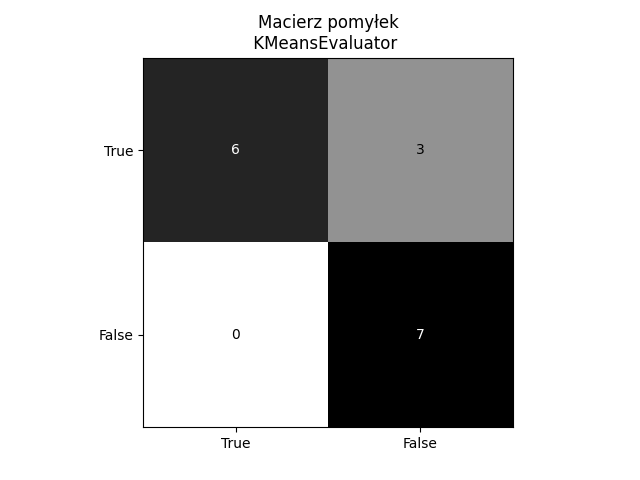
\includegraphics
            [width=\textwidth,keepaspectratio]
            {img/chapter5/dataset2/Dellkb522_KMeansEvaluator.png}
            \caption
            [Macierz pomyłek dla zbioru danych \#2, eksperyment \#1]
            {Macierz pomyłek dla zbioru danych \#2, eksperyment \#1}
            \label{fig:chapter5:eksperymenty:zbior:2:eksperyment:1:macierz}
        \end{minipage}
        \hfill
        \begin{minipage}[b]{0.49\textwidth}
            \centering
            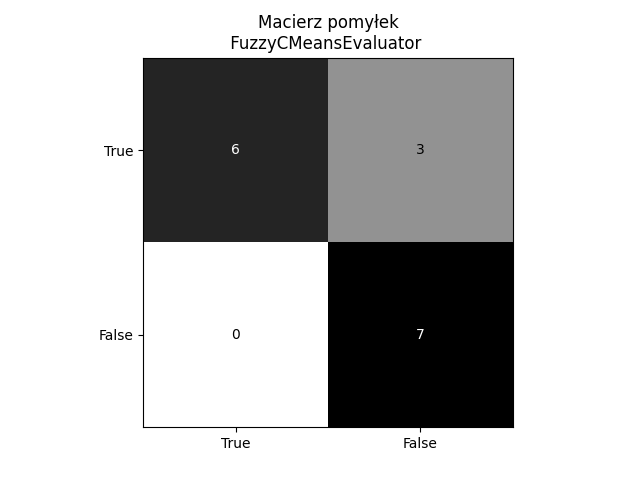
\includegraphics
            [width=\textwidth,keepaspectratio]
            {img/chapter5/dataset2/Dellkb522_FuzzyCMeansEvaluator.png}
            \caption
            [Macierz pomyłek dla zbioru danych \#2, eksperyment \#2]
            {Macierz pomyłek dla zbioru danych \#2, eksperyment \#2}
            \label{fig:chapter5:eksperymenty:zbior:2:eksperyment:2:macierz}
        \end{minipage}
    \end{figure}

    \begin{figure}[H]
        \centering
        \begin{minipage}[b]{0.49\textwidth}
            \centering
            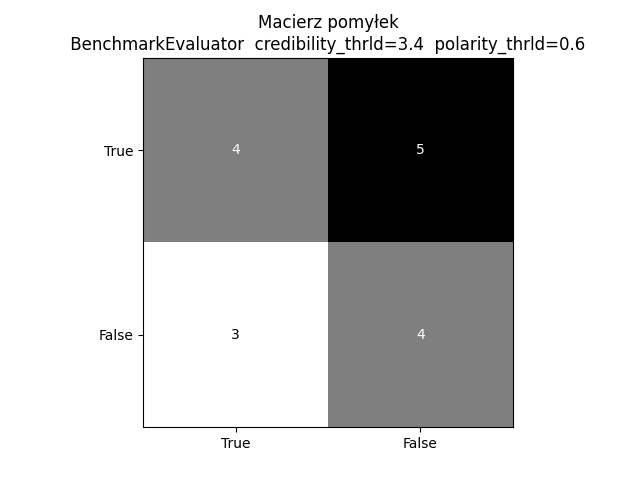
\includegraphics
            [width=\textwidth,keepaspectratio]
            {img/chapter5/dataset2/Dellkb522_BenchmarkEvaluator.png}
            \caption
            [Macierz pomyłek dla zbioru danych \#2, eksperyment \#3]
            {Macierz pomyłek dla zbioru danych \#2, eksperyment \#3}
            \label{fig:chapter5:eksperymenty:zbior:2:eksperyment:3:macierz}
        \end{minipage}
        \hfill
        \begin{minipage}[b]{0.49\textwidth}
            \centering
            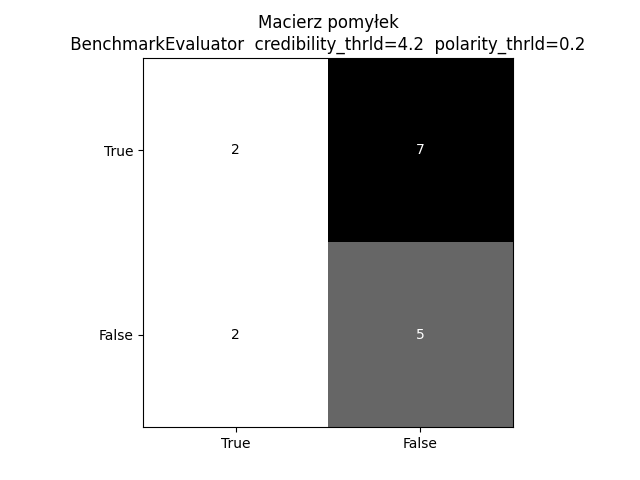
\includegraphics
            [width=\textwidth,keepaspectratio]
            {img/chapter5/dataset2/Dellkb522_BenchmarkEvaluator-1.png}
            \caption
            [Macierz pomyłek dla zbioru danych \#2, eksperyment \#4]
            {Macierz pomyłek dla zbioru danych \#2, eksperyment \#4}
            \label{fig:chapter5:eksperymenty:zbior:2:eksperyment:4:macierz}
        \end{minipage}
    \end{figure}

    \subsection{Podsumowanie uzyskanych wyników}
    \label{chapter5:eksperymenty:zbior:1:podsumowanie} {
        Tak jak w~przypadku zbioru danych \#1 lepsze wyniki zwróciła autorska
        metoda, oba warianty zwróciły takie same wyniki, popełniając 3~błędy
        pierwszego rodzaju. Była za to siedmiokrotna różnica czasu wykonania na korzyść
        metody korzystającej z~C-Means.

        Metoda z~literatury sprawdziła się gorzej, w~eksperymencie \#3 popełniła
        5~błędów pierwszego rodzaju oraz 3~błędy drugiego rodzaju. W~eksperymencie
        \#4 popełniał 7~błędów pierwszego rodzaju i~2~błędy drugiego rodzaju,
        czyli sumarycznie 1~błąd więcej. Czasy wykonania były bardzo zbliżone.
        Można stwierdzić, że skuteczność autorskiej metody jest akceptowalna.
    }

}
\end{document}
